\documentclass[copyright]{tesisunab}

% Borrar esto, pues es solo para texto dummy
\usepackage{lipsum}

% Para poner notas
\usepackage{todonotes}

%INIT--Tables----
\usepackage{multirow}
\usepackage{adjustbox}
%END--Tables----
%INIT--GANTT----
\usepackage{pgfgantt}
\usepackage{xcolor}
\definecolor{barblue}{RGB}{153,204,254}
\definecolor{groupblue}{RGB}{51,102,254}
\definecolor{linkred}{RGB}{165,0,33} 
%END--GANTT----

\title{Neque porro quisquam est qui dolorem ipsum quia dolor sit amet}
\author{Fulano de Tal \and Perengano los Palotes}
\date{\today}

\keywordsEs{Prueba, Tesis}
\keywordsEn{Test, Thesis}

\universidad{universidad andrés bello}
\subtitle{Consectetur, adipisci, velit\ldots}

\facultad{facultad de ingeniería}

\profesor{Mengano}
\profesorco{Sutano}
\propuesta{Trabajo presentado en conformidad a los requisitos para obtener el grado de Magíster xxx}
\ciudad{Santiago}
\pais{Chile}

\copyrightnotice{
	\textcopyright Fulano de Tal, 2023
	
	
\includegraphics[scale=0.25]{./images/ccby.png}
	Algunos  derechos  reservados. Esta  obra  está  bajo  una  Licencia  Creative  Commons  Atribución-Chile  3.0.  Sus  condiciones  de  uso  pueden  ser  revisadas  en:  <\url{http://creative-commons.org/licenses/by/3.0/cl/}>.
}

%\logo{
\includegraphics[scale=.25]{./images/LogoUNAB.png}}

% Archivo de referencias
\addbibresource{referencias.bib}

\begin{document}
	\maketitle

	% ----------------------------------------------------------
	% ----------- PRIMERA PARTE --------------------------------
	% Temas preliminares: abstract, agradecimientos, 
	% dedicatorias...
	\frontmatter
	
	\dedicatoriaSimple{A Lilith, señora de los desposeídos}
	
	\begin{agradecimiento}
		Agradecemos a todos los profesores anónimos de los últimos 10 años que han ido contribuyendo en el tiempo con su experiencia en cada una de estas secciones. Tomar los consejos solo como referencial --- recuerde siempre tomar acuerdos con su profesor guía.
	\end{agradecimiento}
	
	% De acuerdo al formato, lo preliminar termina con las tablas
	% de contenido.	
	\tableofcontents
	\newpage
	%% Indice de tablas
	\listoftables
	\newpage
	%% Indice de figuras
	\listoffigures
	\newpage
	
	\begin{resumenEs}
		\textcolor{red}{Una página ---utilizar la siguiente estructura en el resumen (no más de cinco líneas cada punto): contexto, problema, cómo otros lo han resuelto. en qué han fallado, cuál es la hipótesis de este trabajo, el objetivo, los resultados que se han obtenido (por ahora suponer acorde a lo que uno espera) + contribuciones}
		
		Un buen resumen debe permitir al lector identificar, en forma rápida y precisa, el contenido básico del trabajo; no debe tener más de 200 o 250 palabras y debe redactarse en pasado, escrito en un solo párrafo finalizando con una frase concluyente. No debe aportar información o conclusiones que no está presentes en el texto, así como tampoco debe  citar referencias bibliográficas. Debe quedar claro el problema que se investiga y el objetivo del mismo (lea y analice ejemplos desde artículos publicados, por ejemplo desde \url{www.scielo.org}).
		
		En general, el resumen debe:  
		\begin{itemize}	
			\item Dar contexto al título, plantear el principal objetivo y el alcance de la investigación. \item Describir la metodología empleada.
			\item Dar contexto explicando el tipo o naturaleza de la experiencia, experimento, trabajo o análisis.
			\item Explicitar el principal resultado.
			\item Explicitar la principal conclusión.
		\end{itemize}
	
		Los errores más frecuentes en la redacción del resumen son: 
		\begin{itemize}
			\item No plantear claramente la pregunta, hipótesis u objetivos.
			\item Presentar figuras o esquemas.
			\item Efectuar enumeraciones.
			\item Ser demasiado largo.
			\item Mala redacción y problemas de conceptualización.
		\end{itemize}
	\end{resumenEs}
	
%	\begin{resumenEn}
%		Far far away, behind the word mountains, far from the countries Vokalia and Consonantia, there live the blind texts. Separated they live in Bookmarksgrove right at the coast of the Semantics, a large language ocean. A small river named Duden flows by their place and supplies it with the necessary regelialia. It is a paradisematic country, in which roasted parts of sentences fly into your mouth. Even the all-powerful Pointing has no control about the blind texts it is an almost unorthographic life One day however a small line of blind text by the name of Lorem Ipsum decided to leave for the far World of Grammar. The Big Oxmox advised her not to do so, because there were thousands of bad Commas, wild Question Marks and devious Semikoli, but the Little Blind Text didn’t listen. She packed her seven versalia, put her initial into the belt and made herself on the way. When she reached the first hills of the Italic Mountains, she had a last view back on the skyline of her hometown Bookmarksgrove, the headline of Alphabet Village and the subline of her own road, the Line Lane. Pityful a rethoric question ran over her cheek, then
%	\end{resumenEn}
%	
	% ----------------------------------------------------------
	% ----------- SEGUNDA PARTE --------------------------------
	% Los capítulos pueden ser tantos como haga falta y conviene separarlos, para evitar un 
	% archivo infinitamente largo.
	\mainmatter
	% Archivo de ejemplo para colocar introducción
\chapter{Introducción}
\label{cha:intro}
\todo[inline]{\href{https://es.overleaf.com/learn/latex/Learn\_LaTeX\_in\_30\_minutes}{Learn Latex in 30 minutes}}

\todo{escriba en 3ra persona}

Esta sección debe tener a o menos 2 páginas  y un máximo de 3.

\begin{itemize}
	\item La Introducción es la presentación de una pregunta.
	\item ¿Por qué se ha hecho este trabajo? 
	\item  El interés que tiene en el contexto científico.
	\item  Trabajos previos sobre el tema y qué aspectos no dejan claros, que constituyen el objeto de nuestra investigación.
	\item El penúltimo párrafo de la introducción se utiliza para resumir el objetivo del estudio.
	\item El último párrafo se usa para describir la estructura del documento y lo que se encuentra en cada sección.
\end{itemize}

Dar contexto global al trabajo a realizar, en particular debe ser escrito desde lo no particular, tal que interese al lector. Para efectuar esta sección debe leer o considerar a lo menos 20 artículos indexados (se refiere a artículo publicados en revistas académicas de corriente principal, o congresos). Visite por ejemplo:
\begin{itemize}
	\item \url{www.scielo.org}.
	\item \url{http://www.sciencedirect.com/}.
	\item \url{http://biblioteca.unab.cl/} (debe solicitar su \textit{password} a su coordinador).
\end{itemize}

\todo[inline, color=blue]{Más cómodo en español que en inglés --- solo SoS revíselo en google chrome y active traducción a español. Recuerde que google translate permite subir el pdf del paper también.}

Por favor, considere con ``temor y temblor'' a lo largo de todo el texto las siguientes premisas:
\begin{itemize}
	\item Conecte los párrafos y la secciones a través de las ideas que desarrolla.
	\item Respalde sus afirmaciones con citas. Por ejemplo, si usted dice que el 60 \% de una población es pobre, indique el estudio que respalda dicha afirmación.
	\item Evite redundancia.
	\item No más de dos o tres ideas por párrafo.
	\item Sea asertivo y preciso a la hora de escribir (no sobrevuele, ¡aterrice la idea!).
	\item Debe existir un hilo conductor de ideas claramente definido, no puede saltar de ideas en forma arbitraria.
	\item Todo acrónimo o sigla utilizada debe explicarse la primera vez. Por ejemplo si deseo utilizar la sigla \textsc{``EPTE''}, deberé indicar la primera vez que aparece: Estudiantes de Postgrado Tratando de Escribir (\textsc{``EPTE''}). Luego podrá utilizar la sigla sin mayor mención a su significado. Siempre prefiera versalita para las siglas.
	\item No debe redactar de manera coloquial. Esta debe permanecer alejada del objeto de estudio.
	\item Cuide la concordancia (un concepto debe ser esencialmente el mismo a lo largo de todo el manuscrito).
	\item Cuide los tiempos verbales.
	\item Su trabajo debe ser propio, es decir, debe estar ``limpiamente'' escrito y, además, debe ser suyo. \todo[inline]{Busque referencia de paper: nombre de este y la palabra Bib\TeX ---copie la fuente en formato Bib\TeX y cópielo en su archivo \texttt{.bib}. En la mayoría de los indexadores, es seleccionar la opción ``cite this'' o íconos con carácteres como comillas, entre otros. También los puede construir Ud. Adicionalmente, si bien Bib\TeX sigue siendo utilizado, prefiera su evolución, Bib\LaTeX, que soporta mejor escritura no inglesa y causa menos dolores de cabeza. \href{https://www.overleaf.com/learn/latex/Articles/Getting_started_with_BibLaTeX}{Aquí} hay una introducción.}
\end{itemize}

	% Capítulo de ejemplo para colocar descripción del problema
\chapter{Cuerpo del Trabajo}

\section{Fundamentación}

(1-2 páginas máximo)

Debe explicar cuál es el problema y responder al menos a la pregunta: ¿por qué es importante para usted abordar o resolver el problema que se propone considerar? No olvide mencionar el área, por ejemplo, en \textsc{mcc}: Inteligencia Artificial, Análisis y Minería de Datos o Ingeniería de Software.

\subsection{Ejemplo de citas, tablas}

Es muy importante considerar que el elemento principal para medir calidad en videojuegos es la ``jugabilidad'' y son variados los autores que profundizan en esta definición \parencite{Playability-Quality-Videogames,Metric-Suite-Videogames,Playability-Heuristic,quality-metric-mobile-games}. Montero y González \parencite*{Playability-Quality-Videogames} llevaron a cabo un estudio de la jugabilidad como medida de calidad en videojuegos y definen esta como:

\begin{quote} 
	``El grado en que cada usuario logra metas de juego especificas con efectividad, eficiencia, flexibilidad, seguridad y especialmente satisfacción en el uso del videojuego''
\end{quote}

\begin{table}[hbt]
	\centering
	\begin{adjustbox}{width=1\textwidth}
		\tiny
		\begin{tabular}{cp{2.5cm}p{4cm}clp{2.5cm}}
			\cline{2-6}
			\multicolumn{1}{l}{} & \multicolumn{1}{c}{\textbf{Métrica}} & \multicolumn{1}{c}{\textbf{Propósito}} & \multicolumn{1}{c}{\textbf{Fórmula}} & \multicolumn{1}{c}{\textbf{Interpretación}} & \multicolumn{1}{c}{\textbf{Evaluación}} \\
			\hline
			\multirow{2}{*}{\textbf{Satisfacción}} & Escala de satisfacción & ¿Que tan satisfecho se siente el jugador? & \begin{tabular}[c]{l}f1\\ f2\\ f3\end{tabular} & & Test de usuario + cuestionarios \\
			\cline{2-6}
			& Cuestionario de satisfacción & ¿Que tan satisfecho esta el usuario con características especificas del software? & \begin{tabular}[c]{l}f4\\ f5\\ f6\end{tabular} & & Test de usuario + cuestionario \\
			\cline{2-6}
		\end{tabular}
	\end{adjustbox}
	\caption{Métricas asociadas con los atributos de jugabilidad}
	\label{tab:playability-satisfaction-metrics}
\end{table}

Para este trabajo, se utilizarán como base las metodologías aplicadas en los trabajos de Rodríguez y Corral \parencite*{Rodriguez}, los cuales habla sobre la idoneidad de ``\textsc{lpv}'' para programadores no expertos de robots, y el estudio de Maccormick y Zaman \parencite*{maccormick_zaman_2019} sobre la aplicabilidad de la herramienta de \textsc{lpv}, ``Subvis'', para explorar alternativas en el desarrollo de videojuegos.

Estos estudios evalúan la idoneidad de \textsc{lpv} en entornos o áreas especificas. 

Los autores de los estudios utilizan dos grupos de control, aplicando a uno la herramienta a evaluar y a otro, la herramienta base, para luego aplicar un cuestionario y entrevistas alineadas a las métricas (tabla \ref{tab:playability-satisfaction-metrics}) que cada herramienta u área detectó a un universo o grupo de 10 y 25 usuarios en cada caso, promediando entre los 17 usuarios, numero que se utilizará en este estudio para obtener un grupo valido de datos.

\subsection{Comentarios sobre citas, tablas y figuras}

\begin{figure}[htbp]
	\centering
	\begin{tabular}{|c|c|c|c|c|} \hline
		S & A & T & O & R\\ \hline
		A & R & E & P & O\\ \hline
		T & E & N & E & T\\ \hline
		O & P & E & R & A\\ \hline
		R & O & T & A & S\\ \hline
	\end{tabular}
	
	\caption{Dummy figure}
	\label{fig:dummyfigure1}
\end{figure}

Nótese que las citas deben ir en el formato adecuado (por ejemplo, con paréntesis solo las partes que le corresponden) y las figuras y tablas no interrumpen el flujo del texto, sino que se incluyen como ``flotantes''. Toda referencia a estos, se hacen indicando qué tipo de objeto son (figura, tabla, algoritmo, código, etc.) y su número. Ver, por ejemplo, la figura \ref{fig:dummyfigure1} o las tablas \rangeref{tab:dummytable1}{tab:dummytable3} y la \Fig{fig:dummyfigure1} (estos comandos están definidos en la clase usada para este documento).

\begin{table}[htbp]
	\centering
	\begin{tabular}{|c|c|c|c|c|} \hline
        S & A & T & O & R\\ \hline
        A & R & E & P & O\\ \hline
        T & E & N & E & T\\ \hline
        O & P & E & R & A\\ \hline
        R & O & T & A & S\\ \hline
    \end{tabular}
    
    \caption{Dummy table}
    \label{tab:dummytable1}
\end{table}

En la tabla \ref{tab:dummytable2} usamos un rótulo corto, para no tener el completo en la tabla de contenidos. Por otra parte, la \ref{tab:dummytable3} incluye una referencia bibliográfica dentro de ella.

\begin{table}[hbtp]
	\centering
	\begin{tabular}{|c|c|c|c|c|} \hline
        S & A & T & O & R\\ \hline
        A & R & E & P & O\\ \hline
        T & E & N & E & T\\ \hline
        O & P & E & R & A\\ \hline
        R & O & T & A & S\\ \hline
    \end{tabular}
    
    \caption[Dummy table de nombre largo]{Dummy table con un nombre ridículamente largo, porque a veces estas cosas ocurren y es necesario tratar estos casos, para poder dar un buen ejemplo}
    \label{tab:dummytable2}
\end{table}

\begin{table}[htbp]
	\centering
	\begin{tabular}{|c|c|c|c|c|} \hline
        S & A & T & O & R\\ \hline
        A & R & E & P & O\\ \hline
        T & E & N & E & T\\ \hline
        O & P & E & R & A\\ \hline
        R & O & T & A & S\\ \hline
    \end{tabular}
    
    \caption[Nombre corto]{Otra dummy table \parencite{Navarro-Prieto}.}
    \label{tab:dummytable3}
\end{table}

\subsection{Breve discusión bibliográfica}

(Esta sección debe considerar un mínimo de 4 páginas)

Hasta este momento, el lector de su trabajo  ha visto y considerado el título, con el resumen se ha enterado, entre otros, del objetivo principal, alcance y metodología utilizada, además de los resultados obtenidos con su trabajo. Con la introducción, ha comprendido contexto y desafíos actuales, ha podido analizar el motivo que usted tiene para desarrollar este trabajo, pero es posible que una pregunta interpele a dicho lector y para la cual aún no encuentre respuesta: ¿nadie más ha trabajado antes que usted en este tema?

Para responder a esta pregunta, usted deberá leer o considerar a lo menos 20 artículos indexados (se refiere a artículo publicados en revistas académicas de corriente principal, o congresos), como se dijo en el capítulo \ref{cha:intro}.

Usted, como autor, debe leer, analizar y considerar no solo información, sino también estilos para presentar estudios previos, tal que con ello cimente las bases teóricas que sustentan su propuesta. En esta sección, el trabajo presentado no es suyo, se trata de una recopilación de pensamientos de otros (estado del arte) respecto de un área del conocimiento. Esta recopilación debe ser adecuadamente referenciada (\textbf{Normas APA}). Recuerde que el plagio es un delito, es decir que, si usted utiliza el texto de otro autor y lo copia, es \textbf{plagio}. Si usted utiliza la idea de otro autor y parafrasea ese texto para hacerlo propio y no lo referencia, usted también \textbf{comete plagio}. \todo[inline]{Realice sus entregas mediante blackboard y solicite a su profesor el reporte de originalidad.}

No debe utilizar citas textuales (normalmente entre comillas, ``\ldots''), pues no se trata de la producción de un \textit{collage}. Se trata de que usted lea artículos, sintetice las ideas de otros que le son interesantes y las conecte, tal que de todas ellas pueda usted terminar sentando las bases de la teoría subyacente a su propuesta. Notará usted, entonces, que la clave es leer, evitando los sitios web, las fuentes periodísticas o que carezcan de un adecuado respaldo.

Note usted, como en todo orden de cosas, que su trabajo hereda la calidad de las fuentes utilizadas.
Finalmente, en el último párrafo de esta sección, usted podrá concluir respecto de las áreas que aún no son trabajadas suficientemente, o en las que hay espacios de mejora (según el estado del arte que usted presentó). Desde ahí podrá indicar, por ejemplo, que debido a ello, usted propone la siguiente como contribución de su trabajo (haciendo la conexión que todo lector necesita para entender cabalmente el escrito).

\paragraph{¿Cómo se mide la calidad de mi propuesta?}

Respuesta: La autorregulación es importante, el proyecto le pertenece y usted debe au\-to\-co\-rre\-gir\-se y auto mejorar continuamente. Para ello, la propuesta escrita no debe alejarse significativamente de la calidad de los artículos publicados (mismos que usted considera), luego solo debe compararlos recurrentemente, tanto en forma, fondo y, en particular, su propuesta conceptual.

Usted encontrará discusiones bibliográficas en cada artículo publicado, pero he aquí un breve ejemplo desde la literatura: 

\begin{quote}
	``El uso de este tipo de observadores (del observador Luenberger o Filtro de Kalman), depende de si las perturbaciones son modeladas de forma determinista o estocástica, respectivamente. Además estos algoritmos son  recursivos, es decir, con cada nueva medida calculan el nuevo valor de las variables de estado de acuerdo a una estimación precedente. Una característica fundamental de estos algoritmos es su estabilidad y convergencia; cada nuevo cálculo es más cercano al valor exacto (Kalman y Bucy, 1961), (Luenberger, 1964). Estos resultados estimularon la investigación en los observadores adaptativos para plantas cuyos parámetros no son conocidos (Kudva y Narendra, 1973; Kreisselmeier, 1977). Los observadores adaptativos son usados para proveer estimaciones de los estados de las plantas y estimaciones de los parámetros del sistema simultáneamente (Zhang y Guay, 2002). Aunque el diseño de los observadores adaptativos fue un campo activo de investigación en los años setenta y ochenta, su análisis teórico puede fácilmente llegar a ser altamente complejo (Dochain, 2003).
	
	Si el sistema es no lineal, como es a menudo el caso para los procesos industriales, la situación es más complicada. Las aproximaciones tradicionalmente usadas son la extensión de algoritmos lineales (Sargantinis y Karim, 1994), o algoritmos específicos no lineales (Gauthier et. al., 1992; Farza et. al., 1998). Un ejemplo de la primera aproximación, es la extensión del famoso filtro de Kalman, \textsc{efk} (del inglés, Extended Kalman Filter) el cual es una extensión de la teoría lineal para el dominio no lineal a través de la linealización local (Judd, 2003 y sus referencias). El \textsc{efk} proporciona no sólo estimaciones de las variables de estado, sino también de los parámetros del sistema. Este sistema es un filtro recursivo que incorpora en la estimación los valores estadísticos de los ruidos asociados a los estados y a las medidas. Este observador presenta la ventaja de tratar el sistema de forma más realista, pero a su vez precisa de un mayor cálculo computacional. Este hecho se ha estudiado en (Mora et. al., 2001), donde se destaca que una falla anticipada de este método puede ser constituida por la aproximación local lineal del proceso. De hecho, esta aproximación no garantiza la convergencia y estabilidad (Zhang y Guay, 2002). Es más, el \textsc{efk} necesita del conocimiento estadístico (matrices de covarianza) de los ruidos que actúan en los estados y en la salida, lo cual puede ser difícil de obtener para los casos no lineales (Valdés-González et. al., 2003). Sin embargo, muchas aplicaciones basadas en este tipo de observador se han desarrollado recientemente (ver por ejemplo Cerveri et. al., 2003; Delgado y Barreiro, 2003; Wang y Papageorgiou, 2005)''
\end{quote}

\subsection{Hipótesis}

Si \ldots, entonces \ldots

\subsection{Objetivo General}

(0,5 páginas como máximo)

Debe ser único, en un párrafo y debe estar alineado con el título de la memoria. Que sea \textsc{smart}\footnote{\textit{\foreignlanguage{english}{Specific, Measurable, Assignable, Realistic, Time-bound}}: específico, medible, asignable, realista y temporal (en el sentido de tener un marco temporal para obtener el resultado).}.

\subsection{Objetivos Específicos}

Es la desagregación del objetivo general que describe los pasos sistemáticos y cronológicos a realizar para alcanzar el punto anterior.

Máximo 5 objetivos específicos (todos deben comenzar con verbo en infinitivo, es decir describiendo una acción). Notar que al describir estos verbos como una acción, son al mismo tiempo un compromiso verificable del que se deberá rendir cuenta en las conclusiones. Si, por ejemplo, usted indica en un objetivo específico la necesitar de ``Estudiar un tema'', en las conclusiones será necesario mostrar a través de un párrafo que dicho estudio fue efectuado, logrando con ello alcanzar dicho objetivo. Es decir, se responde a la pregunta que emana desde la acción y que el lector de su trabajo se planteará: ¿habrá logrado el autor alcanzar dicho objetivo? O dicho de manera más simple ¿Estudió ese tema? Esto aplicada para cada objetivo específico.

Que sea \textsc{smart}.

\subsection{Propuesta metodológica}

\begin{figure}[hbtp]
	\centering
	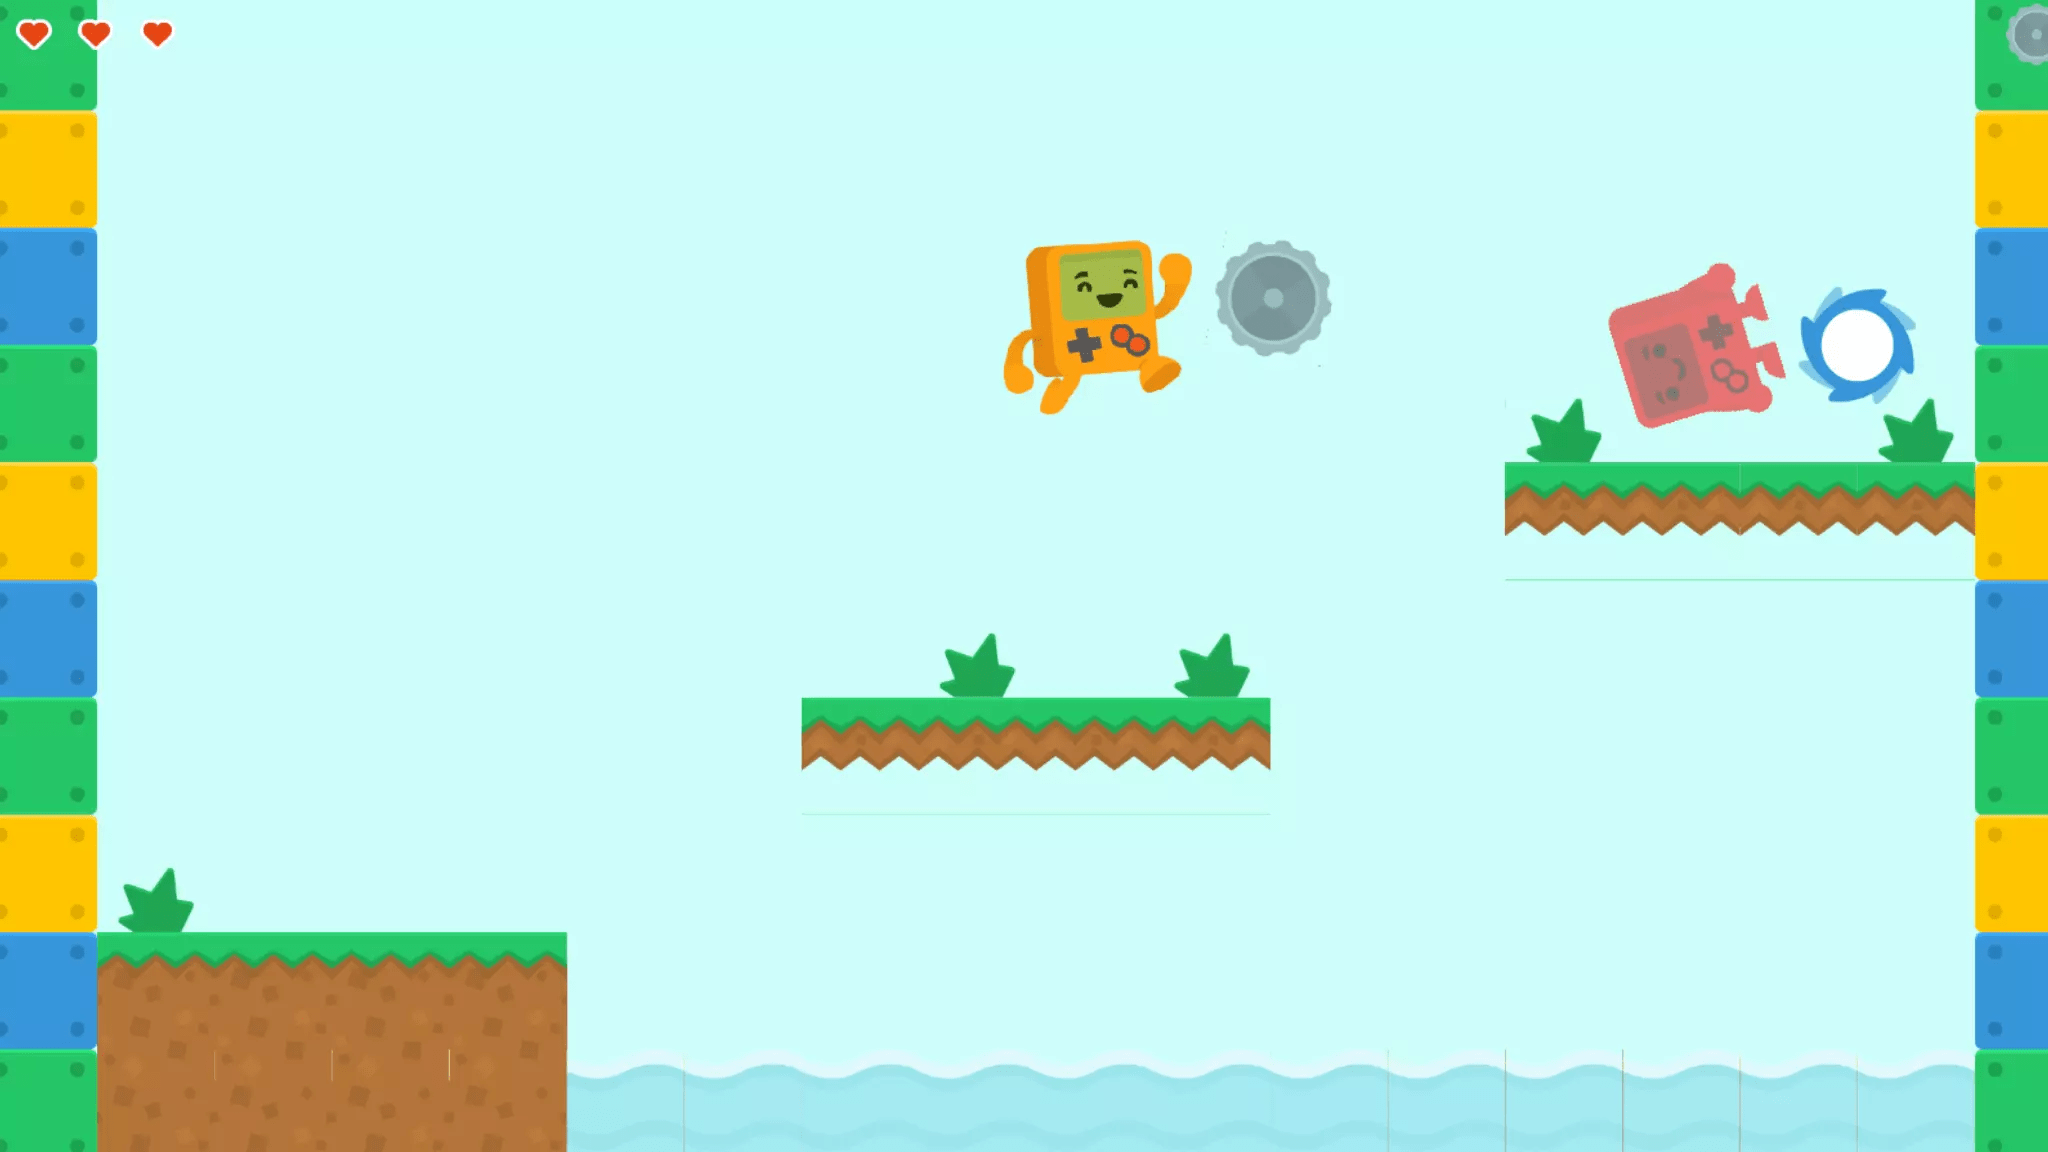
\includegraphics[scale=0.2]{images/gamebase.png}
	\caption{\textsc{¿No es su imagen?} No olvide colocar \textbf{siempre} la fuente: Fuente: Tomás Ramírez o Fuente propia.}
	\label{fig:platformer1}
\end{figure}

Responde a la pregunta de ``cómo se hará el estudio''.  Dicha pregunta no debe extenderse por más allá de 5 páginas.

Jamás olvide la validación de su contribución, considere presentar su metodología respecto las siguientes cinco áreas (si aplica):

\begin{enumerate}
	\item Diseño: se describe el diseño del experimento (aleatorio, controlado, casos y controles, ensayo clínico, prospectivo, etc.).
	\item Población sobre la que se efectuará el estudio. Describe el marco de la muestra y cómo se ha hecho su selección.
	\item Entorno: indica dónde se efectuará el estudio (hospital, asistencia primaria, escuela, etc.).
	\item Intervenciones: se describen las técnicas, tratamientos (utilizar nombres genéricos siempre), mediciones y unidades, pruebas piloto, aparatos y tecnología, etc.
	\item Análisis estadístico: señala los métodos estadísticos utilizados y cómo se han analizado los datos.
\end{enumerate}

En particular, usted debe plantear con detalle y explicar el cómo metodológicamente abordará su propuesta.
Debe quedar claro al final de esta subsección cómo abordará cada objetivo, qué ideas de qué \textit{papers} utilizará más su aporte para resolver cada subproblema.

Usualmente se coloca una pequeña planificación que muestra la calendarización con los principales hitos a lograr. Por ejemplo, la \Fig{fig:Gantt} presenta un ejemplo usando una carta Gantt.

\begin{figure}[hbtp]
    \begin{ganttchart}[vgrid, hgrid]{1}{16}
	        \gantttitlelist{"Sep","Oct","Nov","Dic"}{4}\\
	        \ganttgroup{Proyecto}{1}{16} \\
	        \ganttbar{Creación de herramienta}{1}{4} \\
	        \ganttbar{Iteración de la herramienta}{5}{5} \\
	        \ganttbar{Generación de artefactos}{6}{6} \\
	        \ganttbar{Evaluación artefactos}{7}{8} \\
	        \ganttbar{Procesamiento de datos}{9}{10} \\
	        \ganttbar{Estudio de resultados}{11}{13}
	        \end{ganttchart}
    \caption{Carta Gantt Planificación}
    \label{fig:Gantt}
\end{figure}


\subsection{Contribución del trabajo}

Aquí o al final del capítulo, destacar lo importante, interesante, novedoso o particular de su propuesta, especialmente su aporte. adelante si se cumplió el objetivo general, hipótesis, etc.

En el caso de la descripción del capítulo dos, que para nuestros efectos corresponde a un artículo, usted deberá describir su relación con lo previamente escrito. No olvide indicar dónde fue sometido y su estado actual. Si es más de un artículo, indicar cómo se conectan entre sí. Discutiendo los resultados, explique si se cumple el objetivo general, se refuta o valida la hipótesis, respuestas a la pregunta de investigación, con título de secciones y subsecciones. Qué falta por hacer, qué trabajos futuros podrían derivarse de este trabajo, etc.

(0.5 a 1,5 páginas típicamente, puede ser máximo de una 1 página)

%\subsection{Organización y presentación del trabajo}
%(0,5 páginas)
%Describe el contenido de cada capítulo a partir del segundo, en un párrafo que lo resume y describe en términos generales.

	\chapter{Conclusiones}

Es una parte importante de la tesis o memoria de título donde el autor emite juicios con relación a su
pregunta de investigación o hipótesis, las responde, refuta o comprueba basado en una síntesis de los
resultados obtenidos. Las conclusiones reflejan los alcances y las limitaciones del estudio, las
recomendaciones que puedan ser útiles al ulterior análisis del problema de investigación, así como las consecuencias y determinaciones que puedan contribuir al desarrollo del conocimiento de su campo o
disciplina. Deben presentar una redacción clara, concreta y directas.

Se siguen de las referencias bibliográficas y, si hiciese falta, anexos y apéndices, el material ilustrativo que ayuda a la comprensión detallada del texto, pero que no necesariamente es requerido en el cuerpo de este.

	
	% ----------------------------------------------------------
	% ----------- TERCERA PARTE --------------------------------
	% ### Bibliografía de este documento ###
	% La opción heading la coloca en la tabla de contenidos
	\printbibliography[heading=bibintoc]
	
	\appendix
	\chapter{Addendum}

\lipsum[30]

\begin{table}[hbtp]
	\centering
	\begin{tabular}{|c|c|c|c|c|} \hline
        S & A & T & O & R\\ \hline
        A & R & E & P & O\\ \hline
        T & E & N & E & T\\ \hline
        O & P & E & R & A\\ \hline
        R & O & T & A & S\\ \hline
    \end{tabular}
    
    \caption{Dummy table}
    \label{tab:apptable}
\end{table}

\begin{figure}[hbtp]
	\centering
	\begin{tabular}{|c|c|c|c|c|} \hline
        S & A & T & O & R\\ \hline
        A & R & E & P & O\\ \hline
        T & E & N & E & T\\ \hline
        O & P & E & R & A\\ \hline
        R & O & T & A & S\\ \hline
    \end{tabular}
    
    \caption{Dummy fig}
    \label{fig:appfig}
\end{figure}

\lipsum[31-35]

	
	\annex
	% Por un bug del sistema, si el primer anexo está en un archivo aparte,
	% debe ser incluido con \input, en lugar de \include
	% La excepción a este caso es que después de \annex, se ponga una página
	% en blanco.
	\chapter{Más cosas}

\lipsum[40-45]

	\chapter{Otra porquería}

\lipsum[46-60]
	
\end{document}